\section{Machine Translation with Transformer}

\subsection*{Difference from Transliteration}

(1) many correct translations. (2) locality assumption (scores = $\sum_{\mathrm{arcs}}\mathrm{score}_{i}$) not reasonable.

\subsection*{Seq2Seq Model}

A representation method: $z=\mathrm{encoder}(x)$ and $y\mid x \sim \mathrm{decoder}(z)$. 
Local normalization: $p(y\mid x)=\prod_{t} p(y_t\mid x, y_1, \dots, y_{t-1})$.
Iteratively predict on $p(y_t\mid x, y_1, \dots, y_{t-1})$.  

For standard RNN, the decoder only receives one vector, causing information bottleneck.

\subsection*{Attention Mechanism}

\begin{center}
    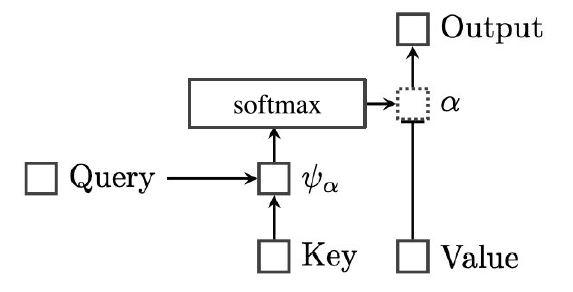
\includegraphics[width=.6\columnwidth]{img/attention.png}
\end{center}
\vspace{-0.5cm}
$Q=W^{Q} X_Q$, $K=W^{K} X_K$,$V=W^{V} X_V$, 

$\mathrm{context}(Q, K, V)=\operatorname{softmax}\left( Q K^{T} / \sqrt{d_{k}}\right) V$

Standard attention: $X_K=X_V=h^{\mathrm{en}}$,$X_Q=h^{\mathrm{dec}}$.

Self-attention: $X_K=X_V=X_Q=h^{\mathrm{en}}$ or $h^{\mathrm{dec}}$.

\subsection*{Decoding}

Beam Search: pruned breadth-first search where the breadth is limited to size $k$.

Sampling: sample according to the conditional distribution at each time step.
